\section{Arhitectura}

Simulatorul rețelelor de transport de date fără fir a fost proiectat pentru a rula pe o singură mașină Linux și să simuleze acolo o topologie de rețea, folosind diferite unelte. Scopul simulatorului a fost să expună în continuare modelele informaționale de bază și pentru microunde, precum versiunea precedentă, \gls{dvm}. Astfel, există un fişier de configurare în care se specifică topologia ce se vrea a fi simulată, în limbajul \textit{Notaţie de Obiecte JavaScript} - \gls{json}. Formatul acestui fişier de topologie este unul fix și este influenţat de către nivelurile de transport ale obiectelor \gls{ltp} definite în modelul informațional de bază. Mai multe detalii despre acest format vor fi date în secţiunea următoare.

Există mai multe unelte care sunt folosite în arhitectura \gls{wte}, care împreună alcătuiesc simulatorul. Fiecare dispozitiv de rețea este simulat printr-un container \textit{docker}, în care rulează o imagine \textit{Linux} și serverul \gls{netconf} reprezentat de \gls{dvm}. Această abordare a fost aleasă pentru a obţine o izolare la nivelul sistemului de fişiere, astfel încât mai mule instanţe ale \gls{dvm} să poată funcţiona fără probleme pe aceeaşi mașină. Interfețele prezente în fiecare echipament sunt reprezentate prin interfețe de rețea în imaginea Linux, iar legăturile dintre dispozitive se fac cu ajutorul acestora. Fiecare element de rețea are o interfață de administrare, prin care se conectează la echipamentul de control \gls{sdn}. Pentru a obţine o izolare a acestor interfețe (mai exact pentru ca traficul de date care ar putea fi transmis prin interfeţele unui dispozitiv să nu tracă prin interfaţa de administrare), astfel încât echipamentele să nu comunice între ele prin aceste interfețe, au fost folosite \textit{rețelele docker}. Toate aceste elemente sunt ilustrare în Figura \ref{fig:wte_architecture} și vor fi detaliate în continuare.

\begin{figure}[h]
	\centering
	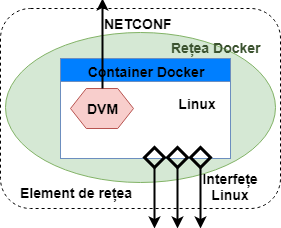
\includegraphics{wte_architecture}
	\caption{Arhitectura WTE.}
	\label{fig:wte_architecture}
\end{figure}

\textit{Docker} este o unealtă care permite crearea de containere software în care pot rula aplicații într-un mod izolat față de aplicațiile sistemului de operare gazdă, care lansează aceste containere \cite{merkel2014docker}. Acestea permit împachetarea unei aplicații într-un container \textit{docker}, împreună cu toate aplicațiile software de care ea depinde. Consumul de resurse al unui astfel de container este mult mai redus decât al unei mașini virtuale, deoarece nu se replică tot sistemul de operare, ci doar bibliotecile și procesele necesare aplicaţiei care este virtualizată. După cum este prezentat și în \cite{chamberlain2014using}, \textit{docker} poate fi utilizat și pentru a produce activitate de cercetare reproductibilă. Astfel, această unealtă este folosită și în cazul \gls{wte} pentru a obţine izolarea, la nivelul sistemului de fişiere al maşinii gazdă, a aplicaţiei ce implementează serverul \gls{netconf} ce expune modelele informaționale dorite: \gls{dvm}.

\textit{Rețelele docker} reprezintă o facilitate oferită de soluţia \textit{docker} prin care se poate izola și stiva de rețea asociată unei imagini \textit{docker}. Astfel, un container poate fi asociat unei \textit{rețele docker} și imaginile ce aparţin unor \textit{rețele docker} diferite sunt izolate și din punctul de vedere al comunicației dintre ele. Un utilizator își poate crea diferite \textit{rețele docker}, având adrese de rețea sau spaţii de adrese la alegere.

Din punctul de vedere al legăturilor ce se pot face între aceste containere, mai exact între interfeţele Linux ce fac parte din imaginile \textit{docker} care reprezintă elementele de rețea, au fost considerate două abordări, după cum se poate vedea în Figura \ref{fig:wte_links}. În prima abordare, s-a încercat folosirea unui comutator software prin intermediul căruia să se facă conexiunile, \textit{Comutatorul Virtual Deschis} - \gls{ovs}. Cea de-a doua abordare constă în crearea unei conexiuni între aceste interfețe printr-o \textit{pereche Ethernet virtuală (virtual ethernet pair - \textbf{veth})}. Diferenţele între cele două abordări vor fi detaliate în secţiunea următoare.

\begin{figure}[h]
	\centering
	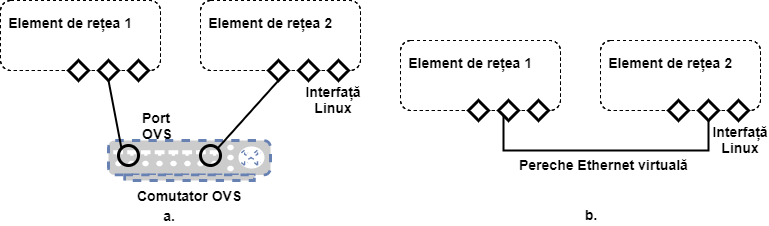
\includegraphics[width=1\textwidth]{wte_links}
	\caption{Legăturile între dispozitivele de rețea simulate în WTE: a) prin OVS; b) prin \textit{veth}.}
	\label{fig:wte_links}
\end{figure}

În urma proiectării \gls{wte} a rezultat o abordare simplă: în momentul inițializării, simulatorul ar trebui să analizeze fişierul care conţine topologia ce trebuie simulată. Apoi, ar trebui să construiască \textit{rețelele docker} asociate fiecărui dispozitiv de rețea definit în topologie și să pornească imaginile \textit{docker} necesare, să creeze interfeţele Linux asociate cu diferitele niveluri de transport ale obiectelor \gls{ltp} definite în topologie, după care să construiască legăturile dintre aceste interfețe.

Componentele care alcătuiesc \gls{wte} sunt prezentate în Figura \ref{fig:wte_components} și sunt următoarele: \gls{dvm}, care a fost adaptat pentru a putea funcţiona în mediul propus de \gls{wte}, fişierul \gls{json} care conţine topologia ce trebuie simulată, fişierul care conţine detalii despre cum ar trebui să fie configurat \gls{wte}, comutatorul software \gls{ovs} (doar în cazul primei abordări propuse pentru reprezentarea legăturilor dintre două elemente de rețea) și un cadru software care să pună toate componentele împreună și să implementeze logica simulatorului. Această ultimă componentă este scrisă în limbajul Python și reprezintă nucleul \gls{wte}.

\begin{figure}[h]
	\centering
	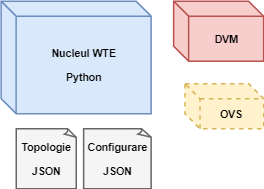
\includegraphics{wte_components}
	\caption{Componentele majore ale WTE.}
	\label{fig:wte_components}
\end{figure}

Nucleul \gls{wte} care este scris în limbajul Python este responsabil pentru implementarea infrastructurii de care simulatorul are nevoie și este proiectat să fie modular și flexibil. Este dezvoltat într-o manieră orientată pe obiecte, având clase pentru fiecare componentă importantă de care este nevoie: cadrul general al simulatorului, elementele de rețea, legăturile de date, topologia, etc. Aceasta oferă posibilitatea de extindere folosind, de exemplu, altă soluție care să implementeze un server \gls{netconf}.